\chapter{Specifikacija programske potpore}
		
	\section{Funkcionalni zahtjevi}
			
			\noindent \textbf{Dionici:}
			
			\begin{packed_enum}
				
				\item Klijent
				\item Administrator				
				\item Razvojni tim
				\item Željezničko poduzeće
				
			\end{packed_enum}
			
			\noindent \textbf{Aktori i njihovi funkcionalni zahtjevi:}
			
			
			\begin{packed_enum}
				\item  \underbar{Neregistrirani korisnik (inicijator) može:}
				
				\begin{packed_enum}
					
					\item se registrirati kako bi se mogao prijaviti u aplikaciju
					
				\end{packed_enum}
			
				\item  \underbar{Klijent (inicijator) može:}
				
				\begin{packed_enum}
					
					\item se prijaviti u stranicu kako bi mogao koristiti aplikaciju
					\item odabrati jedno od ponuđenih stajališta vlaka i dobiti prikaz informacija za svaku ponuđenu vožnju (identifikacijsku oznaku vlaka, krajnje odredište i vrijeme dolaska)
					\item klasično pretražiti red
vožnje u bilo kojem trenutku(odabir mjesta polaska, odabir mjesta dolaska i datum)
					\item kupiti kartu za svaku prikazanu liniju na aplikaciji
					\item obrisati profil/račun
					
				\end{packed_enum}
				
				\item  \underbar{Administrator (inicijator) može:}
				
				\begin{packed_enum}
					
					\item pristupati podatcima o klijentima te pregledati njihove transakcije
					\item pristupati redu vožnje
					\item brisati klijente
					
				\end{packed_enum}				
				
				\item  \underbar{Aplikacija (sudionik) mora:}
				
				\begin{packed_enum}
					
					\item poslati mail s kupljenom kartom klijentu nakon što je klijent plati
					\item poslati drugi mail kojim ga upućuje na određeni kolosijek i peron
					
				\end{packed_enum}
				
				\item  \underbar{Baza podataka (sudionik):}
				
				\begin{packed_enum}
					
					\item pohranjuje podatke o korisnicima i svim njihovim provedenim transakcijama(kupljenim kartama)
					\item pohranjuje podatke o voznom redu, poput polaznog i krajnjeg stajališta, cijene karte, datuma linije i slično
					
				\end{packed_enum}
				
			\end{packed_enum}
			
			\eject 
			
			
				
			\subsection{Obrasci uporabe}
				
				\subsubsection{Opis obrazaca uporabe}

					\noindent \underbar{\textbf{UC1 - Registracija}}
					\begin{packed_item}
	
						\item \textbf{Glavni sudionik: } Korisnik
						\item  \textbf{Cilj:} Stvaranje korisničkog računa za prijavu u sustav
						\item  \textbf{Sudionici:} Baza podataka
						\item  \textbf{Preduvjet:} --
						\item  \textbf{Opis osnovnog tijeka:}
						
						\item[] \begin{packed_enum}
	
							\item Korisnik odabire opciju registracije
							\item Korisnik upisuje potrebne vlastite podatke
							\item Korisnik potvrđuje registraciju
							\item Sustav validira podatke i sprema ih u bazu podataka u slučaju ispravnosti 
							
						\end{packed_enum}
						
						\item  \textbf{Opis mogućih odstupanja:}
						
						\item[] \begin{packed_item}
	
							\item[2.a] Odabir već postojećeg korisničkog imena, odnosno e-maila, upis korisničkog podatka u nedozvoljenom formatu ili pružanje neispravnog formata e-maila
							\item[] \begin{packed_enum}
								
								\item Sustav obavijesti korisnika o neuspješnom upisu podatka i vraća ga na stranicu za registraciju
								\item Korisnik mijenja pogrešne podatke ili odustaje od registracije
								
							\end{packed_enum}
							
						\end{packed_item}
					\end{packed_item}
					
					\noindent \underbar{\textbf{UC2 - Prijava}}
					\begin{packed_item}
	
						\item \textbf{Glavni sudionik: } Klijent, administrator
						\item  \textbf{Cilj:} Prijava za pristup aplikaciji za kupnju karata
						\item  \textbf{Sudionici:} Baza podataka
						\item  \textbf{Preduvjet:} Registracija
						\item  \textbf{Opis osnovnog tijeka:}
						
						\item[] \begin{packed_enum}
	
							\item Korisnik unosi korisničko ime i lozinku
							\item Korisnik potvrđuje navedene podatke
							\item Korisnik dobiva pristup aplikaciji
							
						\end{packed_enum}
						
						\item  \textbf{Opis mogućih odstupanja:}
						
						\item[] \begin{packed_item}
	
							\item[2.a] Neispravno korisničko ime ili lozinka
							\item[] \begin{packed_enum}
								
								\item Sustav obavijesti korisnika o neuspješnoj prijavi i vrati ga na stranicu za prijavu 
								
							\end{packed_enum}
							
						\end{packed_item}
					\end{packed_item}
					
					\noindent \underbar{\textbf{UC3 - Pregled vlakova za stajalište}}
					\begin{packed_item}
	
						\item \textbf{Glavni sudionik: } Klijent
						\item  \textbf{Cilj:} Pregledati sve dolazeće vlakove na stajalište koje je klijent odabrao
						\item  \textbf{Sudionici:} Baza podataka
						\item  \textbf{Preduvjet:} Prijava
						\item  \textbf{Opis osnovnog tijeka:}
						
						\item[] \begin{packed_enum}
	
							\item Korisnik odabire stajalište koje mu treba
							\item Korisnik potvrđuje odabir
							\item Aplikacija prikazuje popis dolazećih vlakova na odabrano stajalište
							
						\end{packed_enum}
						
						\item  \textbf{Opis mogućih odstupanja:}
						
						\item[] \begin{packed_item}
	
							\item[2.a] Korisnik nije odabrao stajalište
							\item[] \begin{packed_enum}
								
								\item Sustav obavijesti korisnika o neuspješnom zahtjevu i zatraži odabir stajališta
								
							\end{packed_enum}
							
						\end{packed_item}
					\end{packed_item}
					
					\noindent \underbar{\textbf{UC4 - Pretraživanje voznog reda}}
					\begin{packed_item}
	
						\item \textbf{Glavni sudionik: } Klijent
						\item  \textbf{Cilj:} Pretražiti vozni red
						\item  \textbf{Sudionici:} Baza podataka
						\item  \textbf{Preduvjet:} Prijava
						\item  \textbf{Opis osnovnog tijeka:}
						
						\item[] \begin{packed_enum}
	
							\item Korisnik odabire mjesto polaska i dolaska
							\item Korisnik odabire željeni datum
							\item Korisnik potvrđuje odabir
							\item Aplikacija prikazuje vozni red za odabrane podatke
							
						\end{packed_enum}
						
						\item  \textbf{Opis mogućih odstupanja:}
						
						\item[] \begin{packed_item}
	
							\item[3.a] Korisnik nije odabrao mjesto polaska, dolaska ili datum
							\item[] \begin{packed_enum}
								
								\item Sustav obavijesti korisnika o neuspješnom zahtjevu i zatraži ponovni odabir i unos
								
							\end{packed_enum}
							
						\end{packed_item}
					\end{packed_item}
					
					\noindent \underbar{\textbf{UC5 - Kupnja karte}}
					\begin{packed_item}
	
						\item \textbf{Glavni sudionik: } Klijent
						\item  \textbf{Cilj:} Kupiti kartu za vlak
						\item  \textbf{Sudionici:} Baza podataka
						\item  \textbf{Preduvjet:} Prijava i pretraga
						\item  \textbf{Opis osnovnog tijeka:}
						
						\item[] \begin{packed_enum}
	
							\item Korisnik odabire vlak za koji želi kupiti kartu
							\item Korisnik upisuje potrebne osobne podatke za kupnju(ime, prezime, podaci o kartici itd.) ili se automatski popunjavaju ako su već upamćeni
							\item Korisnik potvrđuje kupnju
							\item Stizanje 2 e-mailova
							
						\end{packed_enum}
						
						\item  \textbf{Opis mogućih odstupanja:}
						
						\item[] \begin{packed_item}
	
							\item[2.a] Korisnik nije dobro upisao neki podatak
							\item[] \begin{packed_enum}
								
								\item Sustav obavijesti korisnika o neuspješnoj kupnji zbog neispravno unesenih podataka
								\item Korisnik ima mogućnost ponovno unijeti podatke ili odustati od kupnje
								
							\end{packed_enum}
							
						\end{packed_item}
					\end{packed_item}	
					
					\noindent \underbar{\textbf{UC6 - Pregled klijenata}}
					\begin{packed_item}
	
						\item \textbf{Glavni sudionik: } Administrator
						\item  \textbf{Cilj:} Pristupiti i pregledati podatke klijenata
						\item  \textbf{Sudionici:} Baza podataka
						\item  \textbf{Preduvjet:} Korisnik mora biti prijavljen i registriran s dodijeljenim pravom administratora
						\item  \textbf{Opis osnovnog tijeka:}
						
						\item[] \begin{packed_enum}
	
							\item Administrator odabere opciju pregledavanja klijenata
							\item Na aplikaciji se izlistaju podatci svakog korisnika aplikacije
							
						\end{packed_enum}
						
					\end{packed_item}	
					
					\noindent \underbar{\textbf{UC7 - Pregled transakcija}}
					\begin{packed_item}
	
						\item \textbf{Glavni sudionik: } Administrator
						\item  \textbf{Cilj:} Pristupiti i pregledati podatke o provedenim transakcijama
						\item  \textbf{Sudionici:} Baza podataka
						\item  \textbf{Preduvjet:} Korisnik mora biti prijavljen i registriran s dodijeljenim pravom administratora
						\item  \textbf{Opis osnovnog tijeka:}
						
						\item[] \begin{packed_enum}
	
							\item Administrator odabere opciju pregledavanja transakcija
							\item Na aplikaciji se izlistaju podatci svake provedene transakcije kroz aplikaciju
							
						\end{packed_enum}
						
					\end{packed_item}	
					
					\noindent \underbar{\textbf{UC8 - Pregled reda vožnje}}
					\begin{packed_item}
	
						\item \textbf{Glavni sudionik: } Administrator
						\item  \textbf{Cilj:} Pristupiti i pregledati vozni red
						\item  \textbf{Sudionici:} Baza podataka
						\item  \textbf{Preduvjet:} Korisnik mora biti prijavljen i registriran s dodijeljenim pravom administratora
						\item  \textbf{Opis osnovnog tijeka:}
						
						\item[] \begin{packed_enum}
	
							\item Administrator odabere opciju pregledavanja voznog reda
							\item Na aplikaciji se izlista vozni red
							
						\end{packed_enum}
						
					\end{packed_item}

					\noindent \underbar{\textbf{UC9 - Brisanje klijenta}}
					\begin{packed_item}
	
						\item \textbf{Glavni sudionik: } Administrator
						\item  \textbf{Cilj:} Obrisati odabrane korisnike
						\item  \textbf{Sudionici:} Baza podataka
						\item  \textbf{Preduvjet:} Korisnik mora biti prijavljen i registriran s dodijeljenim pravom administratora
						\item  \textbf{Opis osnovnog tijeka:}
						
						\item[] \begin{packed_enum}
	
							\item Administrator odabere klijenta na listi klijenata
							\item Administrator obriše odabranog klijenta opcijom brisanja te potvrdom odluke
							\item Aplikacija ga vraća na osvježenu listu klijenata
							
						\end{packed_enum}
						
					\end{packed_item}	
					
					
						\noindent \underbar{\textbf{UC10 - Odjava}}
					\begin{packed_item}
	
						\item \textbf{Glavni sudionik: } Klijent
						\item  \textbf{Cilj:} Odjaviti se
						\item  \textbf{Sudionici:} 
						\item  \textbf{Preduvjet:} Korisnik mora biti registriran i prijavljen 
						\item  \textbf{Opis osnovnog tijeka:}
						
						\item[] \begin{packed_enum}
	
							\item Klijent zatraži odjavu
							\item Klijentu je obrisana sesija
							\item Klijent je poslan na stranicu za prijavu
							
							
						\end{packed_enum}
						
					\end{packed_item}

					\noindent \underbar{\textbf{UC11 - Brisanje računa}}
					\begin{packed_item}
	
						\item \textbf{Glavni sudionik: } Klijent
						\item  \textbf{Cilj:} Obrisati račun na PassDirect stranici
						\item  \textbf{Sudionici:} Baza podataka
						\item  \textbf{Preduvjet:} Korisnik mora biti prijavljen i registiran
						\item  \textbf{Opis osnovnog tijeka:}
						
						\item[] \begin{packed_enum}
	
							\item Klijent odabire dugme s opcijom brisanja računa na PassDirect stranici
							\item Klijentu se izbaci obavijest s potvrdom brisanja računa, gdje bira između potvrde i odustajanja
							\item Klijent bira opciju
							\item Aplikacija ostane na istoj stranici ako odustane, a ukoliko potvrdi, vraća ga na Login stranicu 
							
						\end{packed_enum}
						
					\end{packed_item}
					
				\subsubsection{Dijagrami obrazaca uporabe}
				
		
		\begin{figure}[H]
			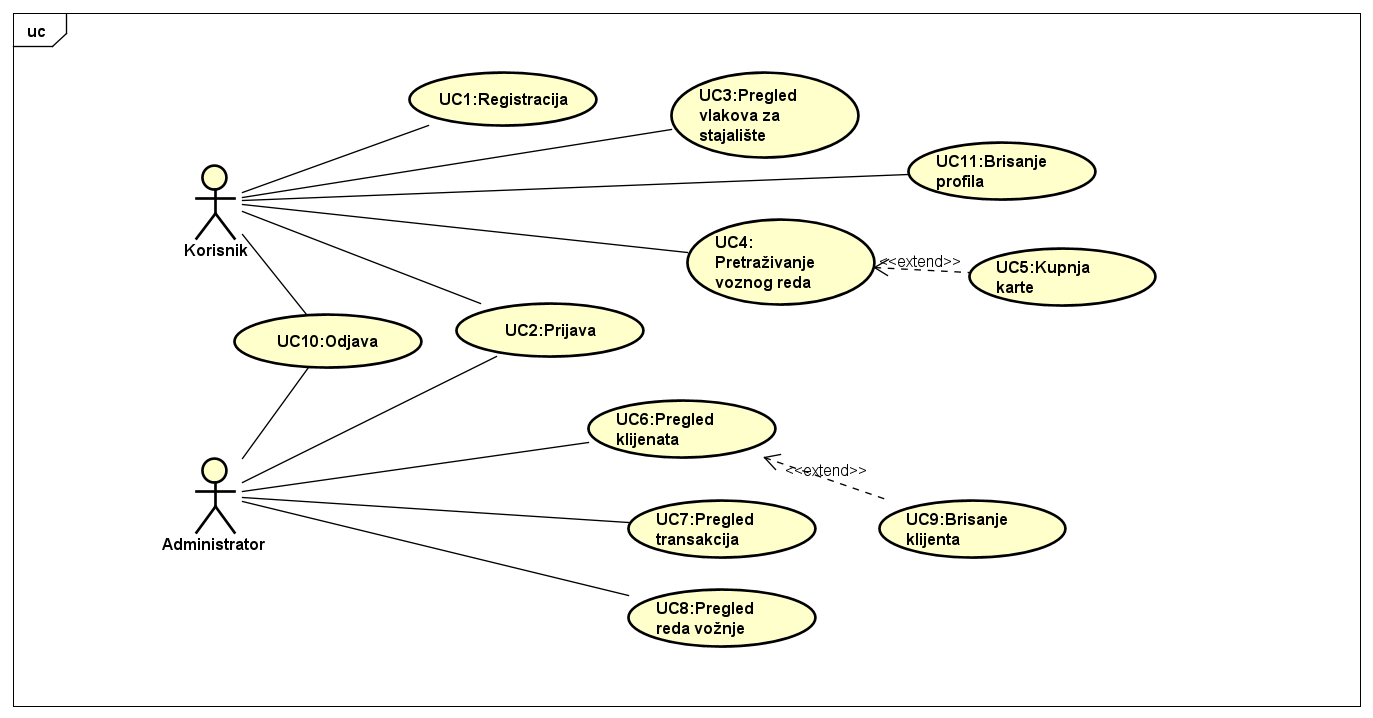
\includegraphics[width=\textwidth]{slike/UCdiagram.PNG} %veličina u odnosu na širinu linije
			\caption{UC dijagram}
			\label{fig:promjene1} %label mora biti drugaciji za svaku sliku
		\end{figure}
				\eject
	
					
				\eject		
				
			\subsection{Sekvencijski dijagrami}

				\noindent \underbar{\textbf{UC3 - Pregled vlakova za stajalište}}\\
				{Klijent odabire i potvrđuje stajalište za koje želi dobiti nadolazeće vlakove. Poslužitelj dohvaća i prikazuje popis i informacije o vlakovima koji stižu na odabrano stajalište.}\\
				
				% TODO: \usepackage{graphicx} required
				\begin{figure}[H]
					\centering
					\includegraphics[width=1\linewidth]{"slike/UC3-sekvencijski"}
					\caption{UC3 - Pregled vlakova za stajalište}
					\label{fig:UC3-pregled-vlakova}
				\end{figure}
		
				\noindent \underbar{\textbf{UC4 - Pretraživanje voznog reda}}\\
				{Klijent odabire mjesto polaska i dolaska te datum polaska, a poslužitelj mu vraća listu mogućih linija za unesene podatke.}\\
				
				% TODO: \usepackage{graphicx} required
				\begin{figure}[H]
					\centering
					\includegraphics[width=1\linewidth]{"slike/UC4-sekvencijski"}
					\caption{UC4 - Pretraživanje voznog reda}
					\label{fig:UC4-pregled-voznog-reda}
				\end{figure}		

				\noindent \underbar{\textbf{UC5 - Kupnja karte}}\\
				{Klijent odabire vlak za koji želi kupiti kartu pa ga poslužitelj odvede na stranicu za checkout. Ovdje unosi sve potrebne podatke za provesti transakciju, nakon čega potvrdi kupnju. Ukoliko su neki podaci netočni ili neispunjeni, poslužitelj daje ponovno mogućnost checkout-a ili odustajanje od kupnje. Kada su podaci točni i ispunjeni, klijentu se javlja uspješna kupnja.}\\
				
				% TODO: \usepackage{graphicx} required
				\begin{figure}[H]
					\centering
					\includegraphics[width=1\linewidth]{"slike/UC5-sekvencijski"}
					\caption{UC5 - Kupnja karte}
					\label{fig:UC5-kupnja-karte}
				\end{figure}	

				\noindent \underbar{\textbf{UC6 - Pregled klijenata}}\\
				{Administrator odabire opciju pregleda podataka o svim klijentima. Poslužitelj dohvaća i prikazuje popis i informacije o klijentima.}\\
				
				% TODO: \usepackage{graphicx} required
				\begin{figure}[H]
					\centering
					\includegraphics[width=1\linewidth]{"slike/UC6-sekvencijski"}
					\caption{UC6 - Pregled klijenata}
					\label{fig:UC-pregled-klijenata}
				\end{figure}

				\noindent \underbar{\textbf{UC7 - Pregled transakcija}}\\
				{Administrator odabire opciju pregleda podataka o svim provedenim transakcijama. Poslužitelj dohvaća i prikazuje popis i informacije o svim provedenim kupnjama karata.}\\
				
				% TODO: \usepackage{graphicx} required
				\begin{figure}[H]
					\centering
					\includegraphics[width=1\linewidth]{"slike/UC7-sekvencijski"}
					\caption{UC7 - Pregled transakcija}
					\label{fig:UC-pregled-transakcija}
				\end{figure}

				\noindent \underbar{\textbf{UC8 - Pregled reda vožnje}}\\
				{Administrator odabire opciju pregleda podataka o voznom redu, odnosno linijama vlakova. Poslužitelj dohvaća i prikazuje popis i informacije o svim voznim linijama vlakova.}\\
				
				% TODO: \usepackage{graphicx} required
				\begin{figure}[H]
					\centering
					\includegraphics[width=1\linewidth]{"slike/UC8-sekvencijski"}
					\caption{UC8 - Pregled voznog reda}
					\label{fig:UC-pregled-voznog-reda}
				\end{figure}

				\noindent \underbar{\textbf{UC9 - Brisanje klijenta}}\\
				{Administrator odabire klijenta te mu se izbacuje opcija za brisanje odabranog klijenta. Nakon odabira opcije, poslužitelj briše klijenta i vraća administratora na osvježenu listu klijenata.}\\
				
				% TODO: \usepackage{graphicx} required
				\begin{figure}[H]
					\centering
					\includegraphics[width=1\linewidth]{"slike/UC9-sekvencijski"}
					\caption{UC9 - Brisanje klijenta}
					\label{fig:UC-brisanje-klijenta}
				\end{figure}

				\noindent \underbar{\textbf{UC11 - Brisanje računa}}\\
				{Klijent odabire opciju brisanja računa u zaglavlju stranice. Web-aplikacija mu izbaci notifikaciju s upitom o potvrdi brisanja računa. Ukoliko klijent potvrdi, aplikacija ga vrati na Login stranicu, a u slučaju da odustane od brisanja računa, ostane na stranici na kojoj je bio. }\\
				
				% TODO: \usepackage{graphicx} required
				\begin{figure}[H]
					\centering
					\includegraphics[width=1\linewidth]{"slike/UC11-sekvencijski"}
					\caption{UC11 - Brisanje računa}
					\label{fig:UC-brisanje-racuna}
				\end{figure}
				
				
		\section{Ostali zahtjevi}
		
			\begin{packed_item}
				\item {Sustav treba omogućiti rad više korisnika u isto vrijeme.}
				\item {Sustav mora biti izveden kao web aplikacija s objektno orijentiranim jezikom.}
				\item {Komunikacija između korisnika i sustava mora biti brza i jednostavna.}
				\item {Aplikacija mora prikazivati aktualne, odnosno ažurirane podatke u svakom trenutku.}
				\item {Aplikacija mora raditi u stvarnom vremenu.}
				\item {Sustav kao valutu koristi HRK.}
				\item{Baza podataka treba biti brza, učinkovita i dobro povezana sa sustavom, otporna na bilo kakve greške korisnika i administratora.}
				\item {U slučaju pogrešaka ili zlonamjernih unosa od strane korisnika, sustav mora izbaciti odgovarajuće upozorenje}
					\begin{packed_item}
					\item {U slučaju lozinke kraće od 6 znakova, izbaci se obavijest da je nužno barem 6 znakova.}
					\item {Ukoliko neki od podataka koji se moraju ispuniti nisu ispunjeni, izbaci se upozorenje o tome.}
					\item {Prilikom prijave ili registracije netočnim podacima, također se ispisuje upozorenje o tome.}
					\end{packed_item}
				\item {Dodatna poboljšanja(senzor za pomoć očuvanju vagona) ne smiju ugroziti već postojeće osnovne funkcionalnosti aplikacije.}
				\item {Korisnik jednim mailom može otvoriti samo jedan račun na stranici.}
				\item {Aplikacija mora automatski popunjavati informacije u korisniku pri kupnji karata.}
			\end{packed_item}
		 
			 
			 
			 
	